\chapter{Theory}\label{chapter:theory}

The theory relating to this work is can be split into two halfs: stellar spectroscopy and binary stars. The former relates to the atmospheric parameters which can be measured using specific absorption lines from a star's spectrum. The theory surrounding binary stars relates to Kepler's equations and how they can be solved to calculate models for transit photometry and radial velocities. 

\section{Stellar spectroscopy}

The atmospheres of FGK stars are significantly hotter than M-dwarfs and so have a much lower abundance of molecules in the photosphere. Consequently, atmospheric models for FGK stars are well understood and allow for accurate measurements of mass and radius from photometry and spectroscopy alone. In the following sections I will give a basic description of the atmospheric parameters required for the EBLM analysis ($T_{\rm eff}$ , $\log g$, [Fe/H] and $V \sin i$) and how they are typically measured from a spectrum.

\subsection{Effective temperature}

The effective temperature, $T_{\rm eff}$ , is the apparent temperature of a star \citep{Doyle2015}. The effective temperature is related to the stellar radius, $R_\star$, and luminosity, $L_\star$, via the  Stefan-Boltzmann relationship:
%
\begin{equation}
    T_{\rm eff} = \sqrt[4]{\frac{L_\star}{4 \pi R_\star^2 \sigma_{\rm sb}}},
\end{equation}
% 
where $\sigma_{\rm sb}$ is the Stefan-Boltzmann constant.  Spectral lines can be fitted to give good indications of  $T_{\rm eff}$. A good choice would typically include the Balmer lines, which have almost no gravity dependence for stars below 8000\,K \citep{2008oasp.book.....G}. The H$\alpha$ absorption line is formed just above the convection zone while H$\beta$ forms just within it and parameters obtained from the latter are affected by convection; this causes temperature to be underestimated by around 150\,K \citep{2014MNRAS.444.3592D}. The Balmer lines can also be modelled in non-local thermodynamic equilibrium to account for formation in the hot and diffuse regions of the stellar photosphere. This has the effect of strengthening the core and weakening the core-wing transition changing the derived temperature by 100\,K for H$\alpha$ \citep{Doyle2015}.


\subsection{Broadening processes}

The shape of a spectral line is influenced by processes in the stellar atmosphere. Doppler broadening is caused by random thermally-induced velocities in the photosphere; this Doppler shift creates an uncertainty of the emitted frequency which is Gaussian in nature \citep{2008oasp.book.....G}. A greater effect is atomic collisional broadening where an atom’s electrons energy levels are altered by a collision with a nearby atom. This changes the energy of a photon which can be absorbed by the perturbed atom leading to a broadening effect that is typically greater than its thermal counterpart. On top of all this is the rotational broadening caused by a stars rotation about an axis. Simultaneously observing the whole stellar disk averages the effect of rotation and broadens line profiles.

The presence of velocity fields within the stellar atmosphere has a substantial effect on the shape of spectral lines \citep{Doyle2015}. Solar observations (e.g. \citealt{2009LRSP....6....2N}) and 3D models (e.g. \citealt{2011SoPh..268..255C}) show that turbulence occurs over a broad range of length scales. For 1D models this is parameterised in terms of broadening due to motion on length scales shorter and longer than the mean photon path length. \\

\noindent \textbf{Microturbulence, $\zeta_t$}

Basic atomic modelling fails to reproduce the expected equivalent widths of saturated lines. To circumvent this issue we introduce the adhoc broadening parameter: the microturbulence $\zeta_t$. The size of a microturbulance cell is defined to be less than the mean free path of a photon. Microturbulance broadening is Gaussian in form, has magnitude around 2$\, \rm km\, \rm s^{-1}$ and is added in quadrature with thermal broadening. Introducing $\zeta_t$ can resolve the disagreement of determined abundances using strong and weak lines. To this end, one can determine $\zeta_t$ by plotting equivalent width versus abundance and vary the microturbulence until there is negligible correlation (\citealt{Doyle2015}; \citealt{1984A&A...134..189M}). \\

\noindent \textbf{Macroturbulence, $\nu_{\rm mac}$}

The size of a macroturbulence cell is defined to be more than the optical depth and does not alter the equivalent width of spectral lines. Macroturbulence resembles granulation and acoustic oscillations in the stellar atmosphere (\citealt{Bruntt2010}; Gray 1984).

\subsection{Surface gravity}

Surface gravity is a measure of acceleration due to gravity and usually takes a logarithmic form of Newtons law of gravitation:
%
\begin{equation}
    \log g = \log \left( \frac{M_\star}{M_\odot} \right) - 2 \left( \frac{R_\star}{R_\odot} \right) + \log g_\odot.
\end{equation}
%
By convention this value is quoted in centimeter-gram-seconds units (c.g.s). The constant $\log g_\odot$ ($\approx 4.438$) can be obtained from the IAU system of astronomical constants \citep{2016AJ....152...41P}.  A larger surface gravity results in a higher frequency of atomic collisions which broaden the wings of strong spectral lines. This effect is absent in evolved giants with very large radii, resulting in much narrower lines in the spectra of these stars cf. dwarf stars \citep{2005MSAIS...8..130S}.

By modelling the wings of pressure sensitive lines we can determine log g. A suitable line choice should be stable over a wide temperature range and not blended with other lines. The Na\,I\,D lines at 588.9\,nm and 589.3\,nm persist over a large temperature range along with Mg\,I\,b lines at 516.7\,nm, 517.3\,nm and 518.4\,nm although the magnesium lines can suffer from C$_2$ and MgH absorption \citep{Doyle2015}.

\subsection{Composition}

\begin{figure}
    \centering
    \includegraphics{4-images/balmercurve.jpg}
    \caption{Curve of growth measurements and fit for Balmer line absorption of SDSS J1723+5553. Here the initial rise and the plateau can be seen, but not the second rise due to radiation damping and collisional broadening. Image taken from \protect\citet{2010PASJ...62.1333A}}.
    \label{fig:my_label}
\end{figure}

The abundance of an element in the stellar atmosphere is normally measured relative to the abundance of hydrogen, and can be given on an absolute scale or relative to the Sun. The former is typically quoted as $\log A + 12$ where $A$ is the number ratio of an element to hydrogen in the star, $N_X / N_H$. It is also convenient to express composition relative to the Sun:
%
\begin{equation}
    [X/H] = \log \left( \frac{N_x}{N_H} \right)_\star - \log \left( \frac{N_x}{N_H} \right)_\odot,
\end{equation}
%
where $N_H$ is the number density of hydrogen and $N_X$ is the number density for the star ($\star$) and the Sun ($\odot$). One way to measure composition is to look at the curve-of-growth of equivalent widths for lines of the same species with the following theory: if we consider only a few absorbers in a photospheric region then a line opacity is relatively weak and takes a thermal Doppler form mostly due to the line core region. Here, a plot of $\log (EW)$ V. $\log (N_{\rm absorbers})$ increases linearly (see Fig. 1). As the number of absorbers increase the line core begins to fully absorb the continuum and adding more absorbers does not appreciably increase the EW; the plot of $\log (EW)$ V. $\log (N_{\rm absorbers})$ plateaus. Eventually the line wings begin to add EW due to radiation damping and collisional broadening and our graph begins to rise again with a gradient lower than the first. Measuring the equivalent widths for an element and adjusting the abundance until a theoretical curvature of growth matches the data gives a good handle on abundances in a star. This is the curve of growth method \citep{1995gusu.book.....P}.


\iffalse
\section{Wavelet decomposition of spectra}\label{theory:wavelet_decomp}

Analysis of spectral components at different scales can be done using a discrete wavelet transform (DWT). A DWT tiles the wavelength-scale plane by convolving a spectrum, $f( \lambda )$, with variable sized functions \citep{2012AAS...22033004S}. These functions are called daughter wavelets, $\psi_{\rm a,b}(\lambda)$, which are created from a mother wavelet, $\psi(\lambda )$,  using a shift-and-scale operation,
%
\begin{equation}\label{daugthermother}
\psi_{a,b}(\lambda) = \frac{1}{\sqrt{a}}\psi(\frac{\lambda - b}{a}),\quad a,b \in  \Re, a \neq 0 ,
\end{equation}
%
where  $a$ is a member of the dyadic sequence,
%
\begin{equation}\label{dyadic}
a_{i} = 2^{i}, \quad i = 0,1,2,3,...,n
\end{equation}
%
and $b=kb_{0}$, where $k$ is an integer and $b_0$ is chosen to ensure the recovery of $f(\lambda)$. By employing a DWT, the appropriate values of $b$ are selected to minimise overlap between wavelet convolutions. Following the notation in chapter 8 of \citet{Olkkonen2011}, a discrete wavelet transform can be calculated for each dyadic scale ($i$) and displacement ($k$):
%
\begin{equation}\label{DWT}
WT_{f(\lambda)}(i,k) = \frac{1}{\sqrt{2^i}} \int f(\lambda)\overline{\psi \left(\frac{\lambda - k2^ib_0}{2^i} \right)} d\lambda = f(\lambda),\psi_{i,k}(\lambda)
.\end{equation}
%
The likeness of a wavelet, $\psi_{i,k}$, to a section of the spectrum is given by the wavelet coefficient $WT_{f(\lambda)}(i,k)$ from Eq. (\ref{DWT}). Performing this calculation over the series of dyadic scales and displacements yields wavelet coefficients which represent different sized structures at different wavelengths. I split coefficients into bands with constant scales, $\lbrace WT_{f(\lambda)}(0,b)\rbrace_k$, which represent the likeness of a single scale across the entire spectrum. The power of each scale, $\lbrace WT_{f(\lambda)}(i,b)\rbrace_k^2$ , can be visualised in a power H\"{o}vmoller (one value of $i$ per row) in Fig. \ref{fig:wavelet:wavelet_power}. Bands of coefficients which correspond to noise and low-order continuum artefacts (such as merged \'{e}chelle orders) can then be excluded. A filtered spectrum may be reconstructed with an inverse DWT (IDWT):
%
\begin{equation}\label{IDWT}
f(\lambda) = \sum_{i=-\infty }^{\infty} 2^{\frac{-3i}{2}} \int WT_{f(\lambda)}(i,k)\hat{\psi} \left(\frac{\lambda - b}{2^i} \right)db
,\end{equation}
%
where
%
\begin{equation}
\hat{\psi} \left(\frac{\lambda - b}{2^i} \right) = \frac{\psi \left(\frac{\lambda - b}{2^i} \right)}{\sum_{i=0}^{i=n} \left| \psi \left(\lambda - b \right) \right|^2 }
.\end{equation}
%
The process of reconstructing a spectrum using a subset of wavelet coefficients is called wavelet filtering and is analogous with Fourier filtering. Alternatively, the subset of coefficients may be chosen to meet a threshold criteria (i.e. $\left[ WT_{f(\lambda)}(i,k) \right]^2  \geq \rm 0.01$) which eliminates information that has little contribution to a signal; this is called wavelet compression.
\fi 

















\section{Binary stars}\label{theory:binary_stars}

The position and velocity of each component in a binary system relative to a distant observer are imperative when calculating models of radial velocity and transit photometry. In the following sections I detail how these models are created for a given set of orbital parameters.

\subsection{Positions of binary stars}

\begin{figure}
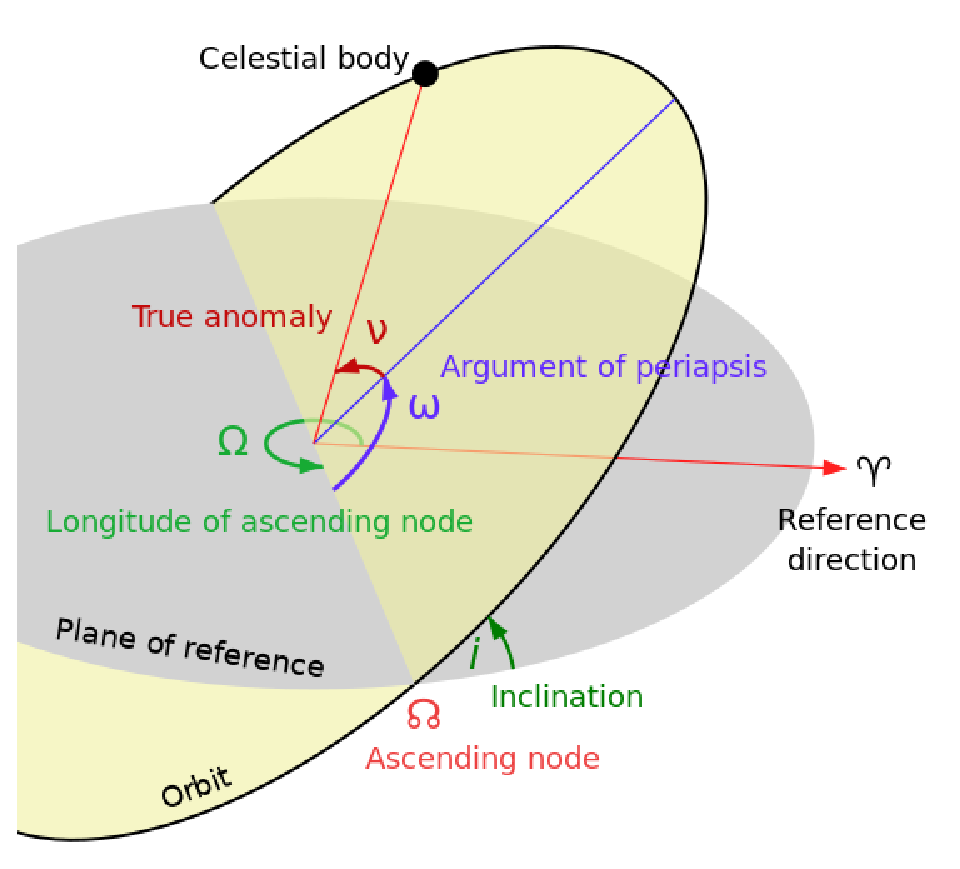
\includegraphics[]{4-images/keplerian_elements}
\caption{Visual representation of Keplerian elements. }
\label{keplerian_elements}
\end{figure}

Johannes Kepler published his first two laws about planetary motion in 1609, having found them by analysing the astronomical observations of Tycho Brahe. They are
%
\begin{enumerate}
    \item All planets move about the Sun in elliptical orbits, where the Sun in one of the foci.
    
    \item A line joining a planet to the Sun sweeps out equal areas in equal lengths of time.
\end{enumerate}
%
Kepler's third law was published later in 1619,
%
\begin{enumerate}
  \setcounter{enumi}{2}
    \item  The squares of the sidereal periods (of revolution) of the planets are directly proportional to the cubes of their mean distances from the Sun. 
\end{enumerate}
%
Any Keplerian trajectory in space can be characterised by a position vector and a velocity vector. Each of these has three components which change through an orbit. It is convenient to instead use \textit{Keplerian elements} - six parameters which can be used to calculate the position and velocity of an orbiting body. Two define the scale and  elongation of the orbit:
%
\begin{itemize}
\item $e$ - eccentricity,
\item $a$ - semi-major axis,
\end{itemize}
%
three define the orientation of the orbital plane:
%
\begin{itemize}
\item $i$ - orbital inclination, the angle between the orbital plane and the reference frame
\item $\Omega$- longitude of the ascending node which defines the angle between the reference direction and the upward crossing of the orbit on the reference plane,
\item $\omega$-argument of periapsis which defines the angle between the ascending node and the periapsis.
\end{itemize}
%
The position of the star(s) at a given time is specified by the following parameter
%
\begin{itemize}
\item $\nu$ - true anomaly which defines the position of the orbiting body along the trajectory, measured from periapsis.
\end{itemize}
%
A visual representation of Keplerian elements can be seen Fig. \ref{keplerian_elements}. The advantage of the Keplerian system over a Cartesian is that only one parameter changes through an orbit - $\nu$.

It is convenient to measure time relative to a reference time, $t_0$, that corresponds to a minimum in sky-projected separation between two stars (conjunction).   At time $t_o$ star 2 is closer to the observer than star 1. The true anomaly of star 1 at this time is $\nu_{1, t_0} \approx \pi /2 - \omega_0$. At other times, $t_i$, the true anomaly requires calculation of the time of periastron passage immediately prior to a given time of eclipse, $t_c$. The mean anomaly can then be calculated,
\begin{equation}
M = 2 \pi \frac{t_i - t_c}{P_a}
\end{equation}
where $P_a$ is the anomalistic period. Keplers law,
\begin{equation}
M = E - e \sin E
\end{equation}
and its differential form,
\begin{equation}
\frac{dM}{dE} = 1 - e \cos E
\end{equation}
can be used to solve for the eccentric anomaly, $E$, using the Newton-Raphson method. The true anomaly can then be calculated for star 1,
\begin{equation}
\nu_1 = 2 \tan ^{-1} \left[   \sqrt{\frac{1 + e}{1 - e}}  \tan (E/2)     \right]
\end{equation}
and $\nu_2 = \nu_1 + \pi$ for star 2. 




\subsection{Radial velocity}

The motion of each component in a binary system relative to the barycentre results in motion projected onto the line of sight. 
%The result is that a spectrum of each component appears more ``blue'' when the projected motion is towards the observer, and ``redder'' when moving in the opposite direction. This is akin to the Doppler effect; the change in pitch of an ambulance siren as it approaches and passes a static observer. 
We can obtain spectroscopic orbital parameters ($e$, $\omega$ and the semi-amplitude, $K_1$) by measuring
%how the spectrum shifts across an orbit. One approach is to measure the wavelength shift of a sharp, unblended line with respect to it’s laboratory wavelength. This provides a measurement of a star’s radial velocity via the Doppler effect equation:
%
%\begin{equation}\label{lambda_vrad}
%\frac{\Delta \lambda}{\lambda_0} = \sqrt{\frac{1 + %\frac{V_{\rm rad}}{c}}{1 - \frac{V_{\rm rad}}{c}}} .
%\end{equation}
%
%Repeating this procedure over many different lines and averaging provides an 
accurate radial velocities at several orbital phases and fitting a Keplerian orbit to these measurements. Another approach is look at the whole spectrum simultaneously. The wavelength shift, $\Delta \lambda$, is a function of radial velocity, $V_{\rm rad}$ , and the rest wavelength of a particular spectral line, $\lambda_0$. Hence an observed spectrum appears to shift by different amounts depending on the wavelength of the line that is measured. One way to overcome this is to convert from a linear wavelength scale to a natural logarithm wavelength scale:
%
\begin{eqnarray}
    \ln \left( \frac{\lambda}{\lambda_0} \right) & = \ln \lambda - \ln \lambda_0 \\
    & \approx \ln \left(1 + \frac{V_{\rm rad}}{c} \right).
\end{eqnarray}
%
Now a radial velocity shift, $V_{\rm rad}$, shifts the spectra along the $\ln \lambda$ axis, proportional to $V_{\rm rad}$ in a manner that is independent of $ \lambda_0$. With this known, we can employ the cross-correlation tool to compare a spectrum to a template spectrum of known radial velocity. A cross correlation is defined:
%
\begin{equation}
    c(x) = \int_{-\infty}^{\infty} f(\lambda) g(\lambda - x) d \lambda
\end{equation}
%
where for the independent variable, $x$, $c(x)$ is equal to the product of the two functions $f$ \& $g$, which are the programme spectrum and a template spectrum respectively. The function $c(x)$ is a measure of how well matched the two functions are over the range of displacement values, $x$. Providing the luminosity ratio between the two stars is not too extreme and the motion of each component along thee line of site is sufficiently different, there will be two peaks in $c(x)$ corresponding to each components moving towards and away from us. In EBLM systems, the FGK star dominates the light and only one peak will be measurable. These type systems which transit are also called single-lined eclipsing binaries (SB1s). It is beneficial to mask spectral features which may broaden/modify $c(x)$. The 8 EBLMs in this work with CORALIE spectra were cross-correlated with a numerical mask\footnote{``Spectrum'' of 0s and 1s at the position of spectral lines.} around Fe lines. The other EBLM with INT spectra masked the core of the H$\alpha$ line. Gaussian functions are often used to fit the peaks in $c(x)$ giving the relative radial velocity motion between the star and the template spectrum.



\begin{figure}
    \centering
    \includegraphics{4-images/radial_velocity_1.png}
    \caption{Example radial velocity models of the primary star for a circular orbit (solid), $e=0.2$ (dashed) and $e=0.4$ (dash-dot). The respective radial velocity models of the secondary stars are shown in light grey.}
    \label{theory:fig:radial_velocity_1}
\end{figure}

Calculating a model for the projected radial velocity ($V_{\rm rad}$) of star 1 at time $t_i$ is trivial once its true anomaly 1 ($\nu_{1,i}$)is calculated,
%
\begin{equation}\label{radial_velocity}
V_{\rm rad} = K_1 \left( e \cos \omega + \cos \nu_{1,i} + \omega \right) + \gamma\:\: \left[+ d(\gamma) / dt\right],
\end{equation}
%
where $K_1$ is the semi-amplitude and $\gamma$ is the systematic velocity of the binary system. Example radial velocity models are shown in Fig. \ref{theory:fig:radial_velocity_1}.  Unresolved faint companions in long-period orbits (tens of years) can introduce drifts in systematic velocity which require an extra term $d(\gamma) / dt$ to account for the inner-binary's orbit around the centre-of-mass. 

The SB1 nature of EBLMs mean that masses of each component cannot be calculated directly. The binary mass function, $f(m)$, can be used to constrain the the mass of the unseen component using parameters from Eqn. \ref{radial_velocity},
%
\begin{equation}\label{mass_function}
f(m)  =  \frac{(M_2 \sin i)^3}{(M_1 + M_2)^2} =  (1-e^2)^{\frac{3}{2}} \frac{P K_1^3}{2 \pi G}.
\end{equation}
%
The orbital inclination is generally not known but can be assumed to be near 90$^\circ$ if the binary system is transiting. In the case of exoplanets, $M_1 + M_2 \approx M_1$ which yields $M_2$ assuming prior knowledge of $M_1$ (e.g. from empirical relations) and inclination. It is important to note that $f(m) \propto K_1^3$ and any uncertainty in $K_1$ propagates by a factor of three into the mass function, and thus the masses of each star/planet. If the spectral lines of both stars can be measured it is possible to calculate the minimum masses of both components,
%
\begin{equation}
M_{1,2} \sin^3 i = c _m(1 - e^2)^{\frac{3}{2}} (K_1 + K_2)^2 K_{2,1} P
\end{equation}
%
where $c_m=1.0361 \times 10^{-7}\,M_\odot$ which is an up-to-date constant from IAU resolution B3 \citep{2016AJ....152...41P}. Similarly, the two semi-major axes of the orbits are,
%
\begin{equation}\label{theory:a}
a_{1,2} \sin i = c_a (1 - e^2)^{\frac{1}{2}}K_{1,2} P
\end{equation}
%
where $c_a = 1.9758 \times 10^{-2}\,R_\odot$.





\subsection{Light-curves}



\begin{figure}
    \centering
    \includegraphics[height=0.8\textheight]{4-images/transit_1.png}
    \caption{The primary eclipse for a uniformly illuminated star (solid), linear limb-darkened star ($c_1 = 0.6$; dashed) and a quadratically limb-darkened star ($c_1 = 0.6$, $c_2 = 0.4$; dash-dot) for impact parameters of $b = 0.0$ (top panel), $b=0.6$ (middle panel) and $b=0.8$ (lower panel). The contact points are marked in the top panel along with ingress/egress regions ($|\delta / R_\star - a| < k$; green) and when the apparent disk of star 2 is entirely encompassed by that of star 1 ($\delta / R_\star < 1-k$; blue). }
    \label{theory:fig:transit_1}
\end{figure}


\begin{figure}
\includegraphics[]{4-images/orbital_seperation}
\caption{The normalised orbital separation in terms of semi-major axis for a circular orbit inclined at $90^{\circ }$ (blue), an orbit with $e = 0.2$ at an inclination of $90^{\circ }$ (green-dashed) and an orbit with $e = 0.2$ at an inclination of $75^{\circ }$ (orange-dashed).}
\label{theory:fig:orbital_seperation}
\end{figure}


Knowledge of the Keplerian elements of an orbit permits the determination of the \textit{sky-projected separation},
%
\begin{equation}\label{sky_projected_seperation}
\delta = \frac{1 - e^2}{1 + e \cos \nu} \sqrt{1 - \sin^2i \sin^2(\nu + \omega)},
\end{equation}
%
where $\delta$ is normalised in terms of the semi-major axis, $a$. At this stage, it is convenient to introduce the radius of star 1 normalised in units of semi-major axis, $R_\star / a$, the ratio of the radii, $k = R_2 / R_\star$, and assume spherical star shapes. Dividing $\delta$ from Eqn. \ref{sky_projected_seperation} by $R_\star / a$ gives the projected sky separation in units of stellar radii. When $\delta / R_\star > 1 + k$, the projected sky-separation of each components disk is such that there is no overlap, and the light from each star is visible. However, when the projected sky-separation is such that $|\delta / R_\star - 1| < k$, there is a partial overlap between the disks of each star. For a primary eclipse (where star 2 is in-front of star 1), this would be the ingress/egress parts of a transit between contact points 1-2, and 3-4 (Fig. \ref{theory:fig:transit_1}). Between contact points 2-3 is where $\delta < 1 - k$ and the disk of star 2 sits entirely within the disk of star 1. 

The calculation of $\delta$ makes no assumption about the absolute position of each star. Over a single period for a transiting binary system, there are two occasions when $|\delta / R_\star - 1| < k$ (Fig. \ref{theory:fig:orbital_seperation}). Determining if a transit is a primary or secondary eclipse requires the calculation of the position for star 1 along the line of sight,
%
\begin{equation}
\bar{l} = \sin{ \left[ 2  \arctan{ \left[ \sqrt{\frac{1 + e}{1 - e}} \tan{\frac{E}{2}} \right] } + \omega \right] } \sin{i} . 
\end{equation} 
%
Instances where $\bar{l} > 0$ are primary eclipses (star 2 in front of star 1) and $\bar{l} < 0$ are secondary eclipses. For systems with low values of $k$, the entirety of the secondary star is obscured in secondary eclipses leading to a flat-bottomed eclipse. The shape of the secondary eclipse is typically parameterised by the surface brightness ratio, $S = k^2 F_{\lambda,2} / F_{\lambda,\star}$, where $F_{\lamda}$ is the flux of each star observed in some bandpass. The depth of a secondary eclipse is then given by $1-S \times k^2$.   


\subsection{Limb darkening}

% look here
% http://iopscience.iop.org/article/10.1086/346105/pdf

\begin{figure}
\includegraphics[scale = 0.5]{4-images/imb_darkening}
\caption{(top) An image obtained from the Solar Dynamics Observatory on March $3^{rd}$ 2018, 01:04:29 UT using the 1700\AA filter. (bottom) The normalised intensity profile of the Sun using the SDO 1700\AA image (top).  }
\label{theory:fig:SDO_1700A}
\end{figure}

Creating a model for an eclipse would be trivial if the disc of each star was uniformly illuminated. In this case, the drop in flux would be proportional the area occulted on the furthest star by the nearest star. This would result in transits where all contact points would be easily discernible and the flux between contact points 2 and 3 would be constant. Unfortunately,  lightcurves taken in filters blueward of $\sim 1 \mu m$ show a slight ``rounding'' of the lightcurve caused by stars emitting more light at the centre than the edge (limb); this is called limb darkening. The reason for this is that light occulted near the limbs originates from a colder column of gas which emits less light than a hotter column of gas near the centre of the disk. This can be seei in an image of the Sun from the Solar Dynamics Observatory (Fig. \ref{theory:fig:SDO_1700A}) which shows a clear drop in light emmited toward the edge of the solar disk.  This intensity across a stellar disk is typically defined in terms of $\mu = \cos \gamma$, where $\gamma$ is the angle between a line normal to the stellar surface and the line of sight. How the normalised intensity $I(\mu)/I_0$ is related to $\mu$ largely remains a task for theoreticians since very few stars are resolvable (see Altair \citealt{2007Sci...317..342M}; $\pi^1$ Gruis \citealt{2018Natur.553..310P}; Betelgeuse \citealt{1998AJ....116.2501U}; Antares \citealt{2017Natur.548..310O} \ldots) and provide little or no constraints on surface intensity distributions across different spectral types.

As stated by \citet{2002astro.ph.10076S}, the generel effect of limb darkening is to (1) change the depth of the lightcurve as a function of impact parameter, where the transit is deeper for most values of impact parameter, (2) make the flat bottom between contact points 2 and 3 rounder and (3) blur the boundary between contact points 2 and 3. These effects are show in Fig. \ref{theory:fig:transit_1}. There are a number of limb-darkening laws used to describe how $I(\mu)/I_0$ changes with $\mu$. These largely depend on a series of coefficients, $c_i$, depending on the number of parameters. Some examples are,
%
\begin{eqnarray}
I(\mu)/I_0 & = 1 - c_1(1 - \mu) & \rm [Linear]\footnotemark\\
I(\mu)/I_0 & = 1-c_1(1-\mu) - c_2(1 - \mu)^2 & \rm [quadratic]\footnotemark \\
I(\mu)/I_0 & = 1 - c_1 (1 - \mu) - c_2 (1 - \sqrt{\mu}) & \rm [square \text{-} \rm root]\footnotemark \\
I(\mu)/I_0 & = 1 - c_1 (1 - \mu) - c_2 \mu \log \mu & \rm [logarithmic]\footnotemark \\
I(\mu)/I_0 & = 1 - c_1 ( 1 - \mu) - \frac{c_2}{1 - \exp{\mu}} & \rm [exponential]\footnotemark \\
I(\mu)/I_0 & = 1 - c_1 (1 - \mu) - c_2 ( 1 - \mu^{\frac{3}{2}}) - c_3 (1 - \mu^2) & \rm [sing]\footnotemark \\
I(\mu)/I_0 & = 1 - c_1 (1 - \mu^{c_2}) & \rm [power \text{-} \rm 2]\footnotemark \\
I(\mu)/I_0 & = 1 - c_1(1 - \mu^{\frac{1}{2}}) - c_2 (1 - \mu) - c_3 (1 - \mu^{\frac{3}{2}}) - c_4 (1 - \mu^2) & \rm [claret]\footnotemark .
\end{eqnarray}
%
\addtocounter{footnote}{-7}
\footnotetext{\citet{1906MiGoe..13....1S}}
\stepcounter{footnote}
\footnotetext{\citet{1950HarCi.454....1K}}
\stepcounter{footnote}
\footnotetext{\citet{1992A&A...259..227D}}
\stepcounter{footnote}
\footnotetext{\citet{1970AJ.....75..175K}}
\stepcounter{footnote}
\footnotetext{\citet{2003A&A...412..241C}}
\stepcounter{footnote}
\footnotetext{\citet{2009A&A...505..891S}}
\stepcounter{footnote}
\footnotetext{\citet{1997A&A...327..199H}}
\stepcounter{footnote}
\footnotetext{\citet{Claret2000}}
%
Many of these limb-darkening laws have tables of coefficients ($c_i$) for a given set of stellar atmospheric parameters ($T_{\rm eff}$, [Fe/H] and $\log g$). I used the Claret 4-parameter law to fit the lightcurves of 5 EBLMs observed from ground-based instruments by interpolating coefficients for a given limb-darkneing temperature. I used the power-2 law to measure 4 EBLMs observed with K2 by fitting the coefficients, $c_i$, as free parameters (see Sect. \ref{method:orbital_fit}). To model secondary eclipses I assumed that the M-dwarf is uniformly illuminated and use the analytical expression presented by \citet{2015PASP..127.1161K}. 


\section{Absolute parameters}

Transit photometry parameters ($R_\star / a$, $k$ \& $i$) sets the radii scale of the system whilst radial velocity parameters ($K_1$ \& $e$) set the mass scale between the components. Often, we are more interested in dimensional parameters such as the mass of each companion, or the semi-major axis in astronomical units. For those, the orbital solution (best-fitting transit and radial velocity parameters) must be combined with supplementry information such as the mass or radius of the primary star obtained by other means (e.g. stellar parallax, spectrum or angular diameter; \citealt{2009IAUS..253...99W}). A brief description on how masses, radii and age are interpolated in this work, and across the field, is given in Sect. \ref{methods:eblmmass}. However, two important parameters can be calculated from the orbital solution directly. 

$\log g_2$ of the secondary star can be obtained by combining the mass function (Eqn. \ref{mass_function}) with the mathematical expression of Keplers third law,
%
\begin{equation}\label{Kepler3}
    \frac{P^2}{a^3} = \frac{4 \pi ^2}{G ( M_\star + M_2)},
\end{equation}
%
it is possible to solve for the sum of the masses of the two components,
%
\begin{equation}\label{mass_sum}
    (M_\star + M_2)^2 = \frac{2 \pi G M_2^3 \sin^3 i}{(1-e^2)^{3/2} K_1^3 P} = \frac{(2 \pi)^4 a^6}{G^2 P^4}.
\end{equation}
%
By substituting $R_2 = a r_2$, where $r_2 = R_2 / a$, into the definition of surface gravity and replacing $a$ using Eqn. \ref{mass_sum}, the surface gravity of star 2 can be calculated:
%
\begin{equation}\label{suface_gravity}
    g_2 = \frac{2 \pi}{P} \frac{\sqrt{1 - e^2} K_1}{r_2^2 \sin i}.
\end{equation}
%


Density of the primary star, $\rho_\star$, can also be calculated from the total transit duration assuming a circular orbit,
%
\begin{equation}\label{transit_duration}
    t_T = \frac{P}{\pi} \arcsin \left( \frac{R_\star}{a} \sqrt{\frac{(1 + k)^2 - b^2}{1 - \cos^2 i}} \right).
\end{equation}
%
By combining Eqn. \ref{Kepler3} with Eqn. \ref{transit_duration} it is possible to calculate the stellar density,
%
\begin{equation}\label{mean_density}
    \rho_\star \equiv \frac{M_\star}{\frac{4}{3} \pi R_\star^3} = \frac{3 \pi}{G P^2} \left( \frac{a}{R_\star} \right)^3 - \frac{M_2}{R_\star^3}.
\end{equation}
%
For exoplanets ($M_\star >> M_2$), the second term on the right-hand side of Eqn. \ref{mean_density} can be ignored to give a robust estimate of the stellar density. For EBLMs systems, the mass ratio $q = M_2 / M_\star \approx 0.1$-$0.6$ and so Eqn. \ref{mean_density} requires further constraints on masses and radii. 

